% Manuscripts for Research articles submitted to The Journal of Pathology Informatics should be divided into the following sections:
% Title page - This should include the title of the article, as well as the full names, institutional addresses, and e-mail addresses for all authors. Indicate which author will be the corresponding author.
% Abstract - The abstract should be around 350 words and must be structured containing into separate sections (background, methods, results, conclusions).
% Background - The context and purpose of the study.
% Methods - How the study was performed.
% Results – Report of study findings.
% Conclusions - Brief summary and potential implications.
% Competing interests
% Authors' contributions
% Acknowledgements
% References
% Figure legends (if any)
% Tables and captions (if any)
% Description of additional data files (if any)

\documentclass[review]{elsarticle}

\usepackage{lineno,hyperref}

% \hypersetup{colorlinks,urlcolor=blue}

\modulolinenumbers[5]

% Custom package imports
\usepackage{booktabs}
\usepackage{subcaption}

\usepackage[acronym]{glossaries}

\usepackage{tikz}
\usetikzlibrary{positioning}

\usepackage{tikzit_setup/tikzit}
\input{tikzit_setup/tikzit_styles.tikzstyles}

\newacronym{wsi}{WSI}{Whole Slide Image}
\newacronym{psnr}{PSNR}{Peak Signal to Noise Ratio}
\newacronym{ssim}{ssim}{Structural Similarity}
\newacronym{jpeg}{JPEG}{Joint Photographic Experts Group}
\newacronym{vqvae}{VQVAE}{Vector Quantised Variational Autoencoder 2 variant}
\newacronym{vae}{VAE}{Variational Autoencoder}
\newacronym{autoencoder}{AE}{autoencoder}
\newacronym{cam16}{$DS_{1}$}{Camelyon 2016}
\newacronym{ucla}{$DS_{2}$}{University of California}
\newacronym{intvalset}{$DS_{3}$}{Internal Validation Set}
\newacronym{comprat}{CR}{Compression Ratio}
\newacronym{mean}{$\mu$}{mean}
\newacronym{stddev}{$\sigma$}{standard deviation}
\newacronym{cnn}{CNN}{convolutional neural network}
\newacronym{exif}{EXIF}{Exchangeable image file format}

\journal{Journal of Pathology Informatics}

%%%%%%%%%%%%%%%%%%%%%%%
%% Elsevier bibliography styles
%%%%%%%%%%%%%%%%%%%%%%%
%% To change the style, put a % in front of the second line of the current style and
%% remove the % from the second line of the style you would like to use.
%%%%%%%%%%%%%%%%%%%%%%%

%% Numbered
%\bibliographystyle{model1-num-names}

%% Numbered without titles
%\bibliographystyle{model1a-num-names}

%% Harvard
%\bibliographystyle{model2-names.bst}\biboptions{authoryear}

%% Vancouver numbered
%\usepackage{numcompress}\bibliographystyle{model3-num-names}

%% Vancouver name/year
%\usepackage{numcompress}\bibliographystyle{model4-names}\biboptions{authoryear}

%% APA style
%\bibliographystyle{model5-names}\biboptions{authoryear}

%% AMA style
%\usepackage{numcompress}\bibliographystyle{model6-num-names}

%% `Elsevier LaTeX' style
\bibliographystyle{elsarticle-num}
%%%%%%%%%%%%%%%%%%%%%%%

\begin{document}

\begin{frontmatter}

\title{Digital pathology whole slide image compression with Vector Quantized Variational Autoencoders}
% \tnotetext[mytitlenote]{}

%% Group authors per affiliation:
\author[universityOfLeeds,LIDA]{Jason Keighley\corref{correspondingauthor}}% 1,5}
% \ead{ll13jjk@leeds.ac.uk}
\author[universityOfLeeds,CMIV,turingInstitute]{Marc de Kamps} %4,1,6}
\author[universityOfLeeds,LTHT]{Alexander Wright} % 2,1}
\author[universityOfLeeds,LTHT,depClinicalPathSweden]{Darren Treanor} % 1,2,3}


\address[universityOfLeeds]{University of Leeds, Leeds, LS2 9JT, UK}
\address[LTHT]{Leeds Teaching Hospitals NHS Trust, Great George St, Leeds LS1 3EX, UK}
\address[depClinicalPathSweden]{Department of Clinical Pathology, and Department of Clinical and Experimental Medicine, Linköping University, Linköping, Sweden}
\address[CMIV]{Center for Medical Image Science and Visualization (CMIV), Linköping University, Linköping, Sweden}
\address[LIDA]{Leeds Institute for Data Analytics (LIDA), University of Leeds, Leeds}
\address[turingInstitute]{The Alan Turing Institute, London}

% \fntext[universityOfLeeds]{University of Leeds, Leeds, LS2 9JT, UK}
% \fntext[LTHT]{Leeds Teaching Hospitals NHS Trust, Great George St, Leeds LS1 3EX, UK}
% \fntext[depClinicalPathSweden]{Department of Clinical Pathology, and Department of Clinical and Experimental Medicine, Linköping University, Linköping, Sweden}
% \fntext[CMIV]{Center for Medical Image Science and Visualization (CMIV), Linköping University, Linköping, Sweden}
% \fntext[LIDA]{Leeds Institute for Data Analytics (LIDA), University of Leeds, Leeds}
% \fntext[turingInstitute]{The Alan Turing Institute, London}

%% or include affiliations in footnotes:
% \author[mymainaddress,mysecondaryaddress]{Elsevier Inc}
% \ead[url]{www.elsevier.com}

% \author[mysecondaryaddress]{Global Customer Service\corref{mycorrespondingauthor}}
% \cortext[correspondingauthor]{Corresponding author}
% \ead{support@elsevier.com}

% \address[mymainaddress]{University of Leeds, Woodhouse Lane, Leeds, West Yorkshire, LS2 9JT, United Kingdom}
% \address[mysecondaryaddress]{Leeds Teaching Hospitals Trust}

% Abstract - The abstract should be around 350 words and must be structured containing into separate sections (background, methods, results, conclusions).
\begin{abstract}
\paragraph{Background}
Digital pathology \glspl{wsi} are large images ($\sim$30 GB/slide uncompressed) of high resolution (0.25 microns per pixel), presenting a significant data storage challenge for hospitals wishing to adopt digital pathology. Lossy compression has been adopted by scanner manufacturers to address this issue - we compare lossy \gls{jpeg} compression for \glspl{wsi} and investigate the \gls{vqvae} as a possible alternative to reduce file size while encoding useful features in the compressed representation.
% This paper contains three novel contributions: a comparison of VQVAE compression performance versus standard pathology compression methods (\gls{jpeg}, \gls{jpeg} with no metadata and \gls{jpeg} 2000 with no metadata); demonstration of generalisability and domain shift of the VQVAE network within \gls{wsi} pathology data and testing of the trained networks on a real-world dataset, to compare performance against existing implementations.
\paragraph{Methods}
We trained three \gls{vqvae} models on a Camelyon 2016 subset to the \gls{comprat} of 19.2:1 ($\gls{comprat}_{1}$), 9.6:1 ($\gls{comprat}_{2}$) and 4.8:1 ($\gls{comprat}_{3}$) and tested on a \gls{cam16} subset; \gls{ucla} and \gls{intvalset}. We then compared compression performance to ImageMagick \gls{jpeg} and \gls{jpeg} 2000 implementations.
\paragraph{Results}
% The \gls{psnr} ($psnr\in R$) for a Camelyon 2016 subset (10 \gls{wsi} slides) and University of California dataset were 28 dB and 28.75 dB for a compression ratio of $\sim$19.2:1 \gls{jpeg} compression with metadata.
\gls{vqvae} compression \glspl{psnr} (\gls{mean}±\gls{stddev}) were 19.6±1.77 dB, 20.3±1.09 dB and 21.49±1.83 dB for \gls{cam16}, \gls{ucla} and \gls{intvalset} respectively. \\
% Structural Similarity (\gls{ssim}) considers image structure, \gls{psnr} does not. \gls{ssim} ($ssim\in[0,1]$) results for the Camelyon 2016 subset and UCLA datasets were 0.35 and 0.35 for \gls{jpeg} with exif data.
The \gls{ssim} was 0.72±0.076, 0.88±0.018 and 0.80±0.060 ($\gls{comprat}_{1}$); 0.75±0.067, 0.87±0.023 and 0.81±0.054 ($\gls{comprat}_{2}$); 0.32±0.12, 0.52±0.039, 0.39±0.13 ($\gls{comprat}_{3}$) for the \gls{vqvae} implementation trained on the \gls{cam16} training data subset (9 \glspl{wsi}). With \gls{jpeg} metadata removed from the compression the \gls{psnr} increased to 30.03±1.34, 32.20±0.89, 30.24±1.31 and the \gls{ssim} increased to 0.88±0.025, 0.87±0.018, 0.84±0.038. \gls{jpeg} 2000 compression without metadata outperformed all other compression methods with the \gls{psnr} and \gls{ssim} being 70.55±4.078, 80.04±2.09, 72.86±3.078 and 0.82±0.082, 0.95±0.015, 0.84±0.064.
\paragraph{Conclusions}
\gls{jpeg} compression outperformed the \gls{vqvae} implementation within the \gls{psnr} and \gls{ssim} metrics. If the \gls{jpeg} metadata was not stripped from the compressed file the \gls{vqvae} implementation outperformed the \gls{jpeg} implementation within the \gls{ssim} metric.
% \gls{ssim} considers image degradation by comparing similar structures within the image and so is a more accurate representation of the overall image reconstruction quality. This suggests the VQVAE compression displays a systematic reconstruction error, whereas the \gls{jpeg} implementation displays a random noise error. A stored transform function within the compressed file may be a possible solution to mitigate the VQVAE reconstruction error.
% Optimising the VQVAE loss function to include the SSIM metric may increase the VQVAE reconstruction accuracy.

\end{abstract}
\begin{keyword}
 Variational Autoencoder \sep Quantisation \sep Compression \sep Pathology \sep Whole Slide Images \sep Digital Pathology
\end{keyword}

\end{frontmatter}

\linenumbers

% Background - The context and purpose of the study.
\section{Background}
\subsection{Introduction}
\paragraph{Digital pathology} Digital pathology is a technology to digitise entire glass pathology slides, allowing the diagnosis of cancer on \glspl{wsi}.\glspl{wsi} allow remote diagnosis of digital images on computer workstations, and viewing of slides by multiple pathologists concurrently, greatly increasing the flexibility and efficiency of tissue diagnosis in cancer compared to glass slides \cite{williams_future-proofing_2017, williams_future-proofing_2019}. However, due to their very high resolution (0.25 microns per pixel, and typical images are 100,000 x 80,000 pixels), causing challenges in the storage and transmission of \glspl{wsi}. To reduce file size, image compression such as \gls{jpeg} 2000 is used by \gls{wsi} scanners, but lossy compression can lead to a reduction in image quality of images depending on the compression ratio applied. This work seeks to investigate the use of alternative compression methods for digital pathology images using \gls{vae}.

\subsection{Related work}
\paragraph{Traditional compression techniques}
In order to enable the scanning of \glspl{wsi}, digital pathology scanners use lossy \gls{jpeg} compression. Although systems attempt to use compression methods that are visually lossless, the of lossy compression in medical imaging is not without issues due to possible information loss \cite{ghazvinian_zanjani_impact_2019}. This information loss can affect the accuracy or consistency of image analysis. Chen et al found that up to 85\% \gls{jpeg} compression would cause a deviation of deep learning algorithms of 95\% compared to uncompressed results within the Camelyon 2017 dataset \cite{chen_quantitative_2020}. Zanjani et al \cite{ghazvinian_zanjani_impact_2019} found similar results, when they trained 3 \gls{cnn} deep learning algorithms on uncompressed images for nucleus segmentation, lymph node metastasis segmentation, and lymphocyte detection tasks. The trained networks were tested on \gls{jpeg} 2000 compressed images with compression around 4\% of their original size. % The network still performed well on the \gls{jpeg} 2000 test images \cite{chen_quantitative_2020}.
In evaluating the effect of \gls{jpeg} compression, metrics such as \gls{psnr} and \gls{ssim} can be used to estimate the impact on image quality. \gls{ssim} has been stated to be better for image comparison within compression, as it takes into account spatial features, rather than comparing pixel to pixel as with \gls{psnr}.

%%% \paragraph{Medical image \gls{autoencoder} compression} \glspl{autoencoder} have been used in many medical image fields. glspl{autoencoder} have been used for two main reasons. The first use is in dimensional reduction or compression. The second use is in extraction of feature representations for clustering or classification.

%%% \paragraph{Medical image deep learning compression} Deep learning algorithms can be used for image compression via the use of encoder-decoder architectures. An encoder can find high level features of an image, and then a decoder can then reconstruct the high-level features back into the original image. More complex encoder-decoder networks can be used. The Encoder can be forced to map the pixels of the input image into a smaller dimensional space, the smaller space representing the high level features of the image. The encoder therefore learns a transformational distribution that converts the pixels to a smaller normally distributed latent feature, $Encoder: X_{ijk} \mapsto Z{m}$ where $X_{ijk} = pixel$; and Z{m} is a vector of size ``m'' with each value representing a normally distributed latent variable. An example of the first Z vector element ($Z{1}\in [-1, 1]$) could represent an image rotation value, with 0 representing 0 degrees and -1 and 1 being a rotation of -180 and 180 degrees respectively.

\paragraph{Medical image \gls{vae} compression} The compression ability of the \glspl{vae} has not been extensively researched to our knowledge, more comprehensive compression research of the \gls{autoencoder} without stochastic sampling has been done \cite{xu_stacked_2016, roy_convolutional_2021, fassler_deep_2020}. \glspl{vae} have a large advantage over \gls{autoencoder} models in real world settings. \glspl{autoencoder} can only generalise latent vectors to previously seen image features. \glspl{vae} map image features to distributions represented within the latent vectors. \glspl{vae} can traverse the probabilistic latent space generating data with similar latent features, \glspl{autoencoder} randomly assign mappings for unencoded latent space, therefore unseen data will be random for each trained \gls{autoencoder} model, reducing model reproducability and reliability, the probabilitstic latent space of \glspl{vae} does not experience this issue due to their probabilistic nature.

%%% \paragraph{VAE latent space representation compression versus traditional compression techniques} No expansive comparison studies between existing VAE latent space representations and traditional compression methods have been done to our knowledge. Most compression-like papers focus on \glspl{autoencoder}, rather than \glspl{vae}.

\paragraph{Proposal of the \gls{vae}} \glspl{autoencoder} have some weaknesses, including the inability to deal with previously unseen data. This means that outside the training datasets, the features identified by the encoder are not stable, and may not represent the actual input data. Networks like \glspl{vae} can combat this by instead of having a latent space vector of values representing the input, the latent space instead represents a distribution. Each distribution represents an approximate learned latent feature; therefore, each latent vector component can use probability distributions to approximate the latent features of unseen data.
This architecture may be able to improve on the shortcomings of glspl{autoencoder}, while not increasing complexity by an incomprehensible amount.

% Methods - How the study was performed.
\section{Materials and methods}
\subsection{Methodology pipeline overview}
\paragraph{Pipeline stages} Data preparation, training of algorithms and testing of algorithms were the three main stages of the methodology pipeline.

% \begin{figure}
% 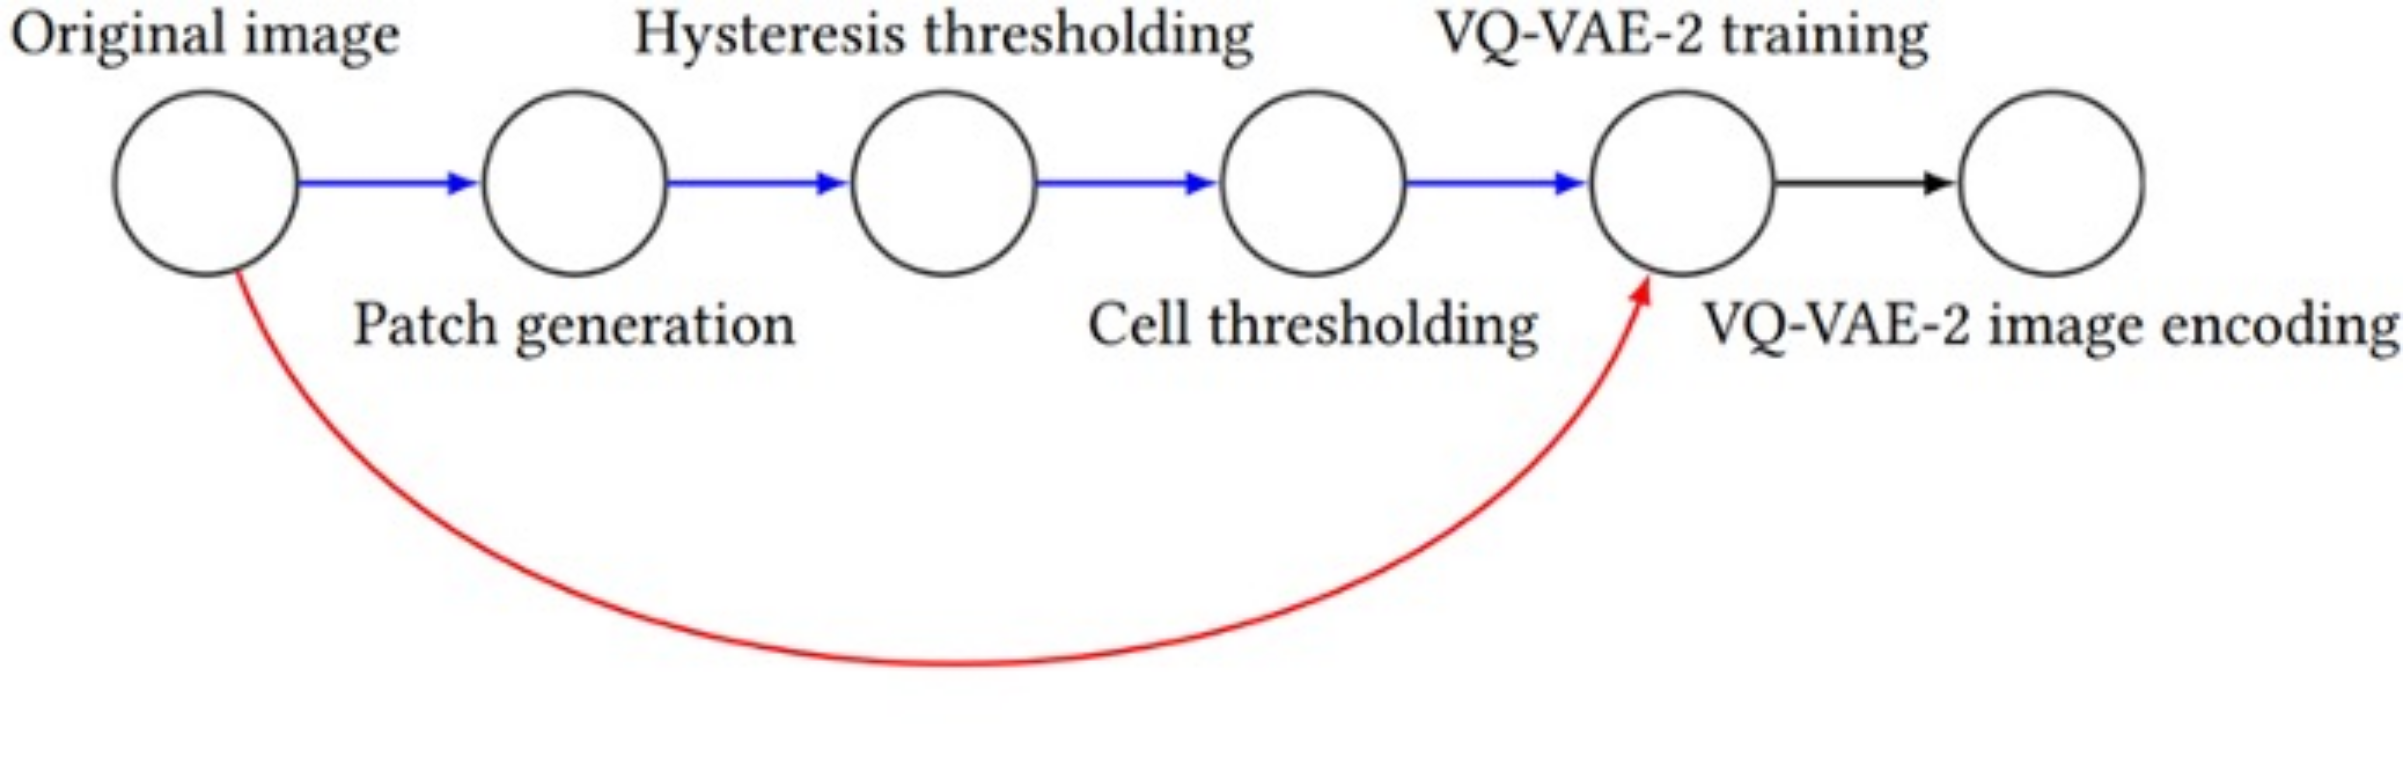
\includegraphics[width=1\linewidth]{Figures/new_500_dpi_figures/Overview VQVAE pipeline.png}
% \caption{Overview of the VQVAE training pipeline}
% \end{figure}

% \begin{figure}
%     \resizebox{\linewidth}{!}{
%         \tikzfig{latex\_figures/Compression VQVAE overview pipeline/Pipeline within VQVAE new pipeline only}
%     }
% \caption{Overview of the Camelyon 2016 data extraction pipeline}
% \end{figure}

\paragraph{Data preprocessing}
We extracted tiles (size=(512, 512, 3), overlap=(12, 12, 0)) from the \gls{cam16} subset dataset, and selected tiles containing tissue samples via hysteresis thresholding.

\paragraph{\gls{vqvae} training}
We trained a \gls{vqvae} at $\gls{comprat}_{1}$, $\gls{comprat}_{2}$ and $\gls{comprat}_{3}$ on a subset of \gls{cam16} thresholded tiles for 500 epochs for each model. We trained a \gls{vqvae} at three \gls{comprat} ($\sim$4.8, $\sim$9.6 and $\sim$19.2) on the thresholded \gls{cam16} patches for 500 epochs, while using a custom data augmentation method which randomises channels to increase model generalise-ability and transfer-ability.

\paragraph{\gls{vqvae} testing}
We tested the trained \gls{vqvae} on the \gls{cam16} subset, \gls{ucla} and \gls{intvalset}. We then tested the trained \glspl{vqvae} with data augmented training data on the \gls{cam16} subset, \gls{ucla} and \gls{intvalset}. We then analysed the generated \gls{ssim} and \gls{psnr} metrics.

\paragraph{\gls{jpeg} compression testing}
We tested the \gls{comprat} (2 to 97 with intervals of 5) for \gls{jpeg} and \gls{jpeg} 2000 compression with and without metadata removed using the --strip function. We then analysed the generated \gls{ssim} and \gls{psnr} metrics.

\subsection{Datasets}
\paragraph{Camelyon 2016 subset} Camelyon was created for cancer segmentation and classification tasks on digital pathology \glspl{wsi}. Originally presented in the Camelyon challenge. The Camelyon dataset was created for two years, creating the \gls{cam16} dataset, and the Camelyon 2017 dataset. The \gls{cam16} dataset is from two hospitals, whereas Camelyon 2017 is from five hospitals. For preliminary experiments on the networks, a subset of the \gls{cam16} dataset was used, containing Normal slides 1-10 (excluding 9) and Cancerous slides (1-10). These \glspl{wsi} were converted to smaller patches for network training and testing.

\paragraph{\gls{ucla}} The \gls{ucla} dataset (n=21 benign, 21 malignant) is a dataset from the University of California. \gls{ucla} consists of \gls{wsi} slide scans, mainly of breast cancer tissue.

\paragraph{\gls{intvalset}} This was a dataset used for internal validation of the algorithms and testing. The \gls{intvalset} consisted of 8,455 512x512x3 patches, which after thresholding was applied became 1,935 512x512x3 patches containing tissue. This dataset allows for testing the models on images from real world data, containing image artefacts.

\subsection{Data preprocessing}
\paragraph{\gls{wsi} patch extraction} OpenSlide was used to extract patches, these patches were 512x512x3 with an overlap of 12. We then used the scikit-image hysteresis thresholding implementation to create a hysteresis threshold map. The hysteresis threshold map was then used to measure the amount of tissue within the patch, with any patch that was over 10\% of the slide being tissue being placed into a thresholded patch set for model training.

\paragraph{Data Augmentation} Data augmentation was used on the training image patches (X) in the form of torchvision.transforms.Compose([torchvision.transforms.Resize((512, 512)), torchvision.transforms.toTensor()]). A custom colour randomising algorithm was also used during \gls{vqvae} training, this used Image:$x_{ijk}\mapsto U\sim(0,2) \times (x_{ijk}); k\in \{0,1,2\}$. A normal distribution can be used as an alternate substitute to the Uniform distribution. Randomising a single channel or multiple channels is another alternative.

\paragraph{Data augmentation reasoning} Within preliminary testing the visual reconstructions showed reconstruction of image structures. \gls{cam16} trained models without data augmentation within preliminary visual testing overfitted to the \gls{cam16} dataset colour palette. The trained models would not generalise to other scanner datasets, reconstructions contained the correct tissue structure but colour similar to the \gls{cam16} dataset. Initial testing of uniform or normal single colour channel scale factors produced a range of colours, trained models learnt from increased colour data allowing for greater model generalise-ability on different datasets. We tested whether this visual difference would affect the quantitative performance of the reconstruction of the images from, the compressed representation.

% \begin{figure}
% \centering
% 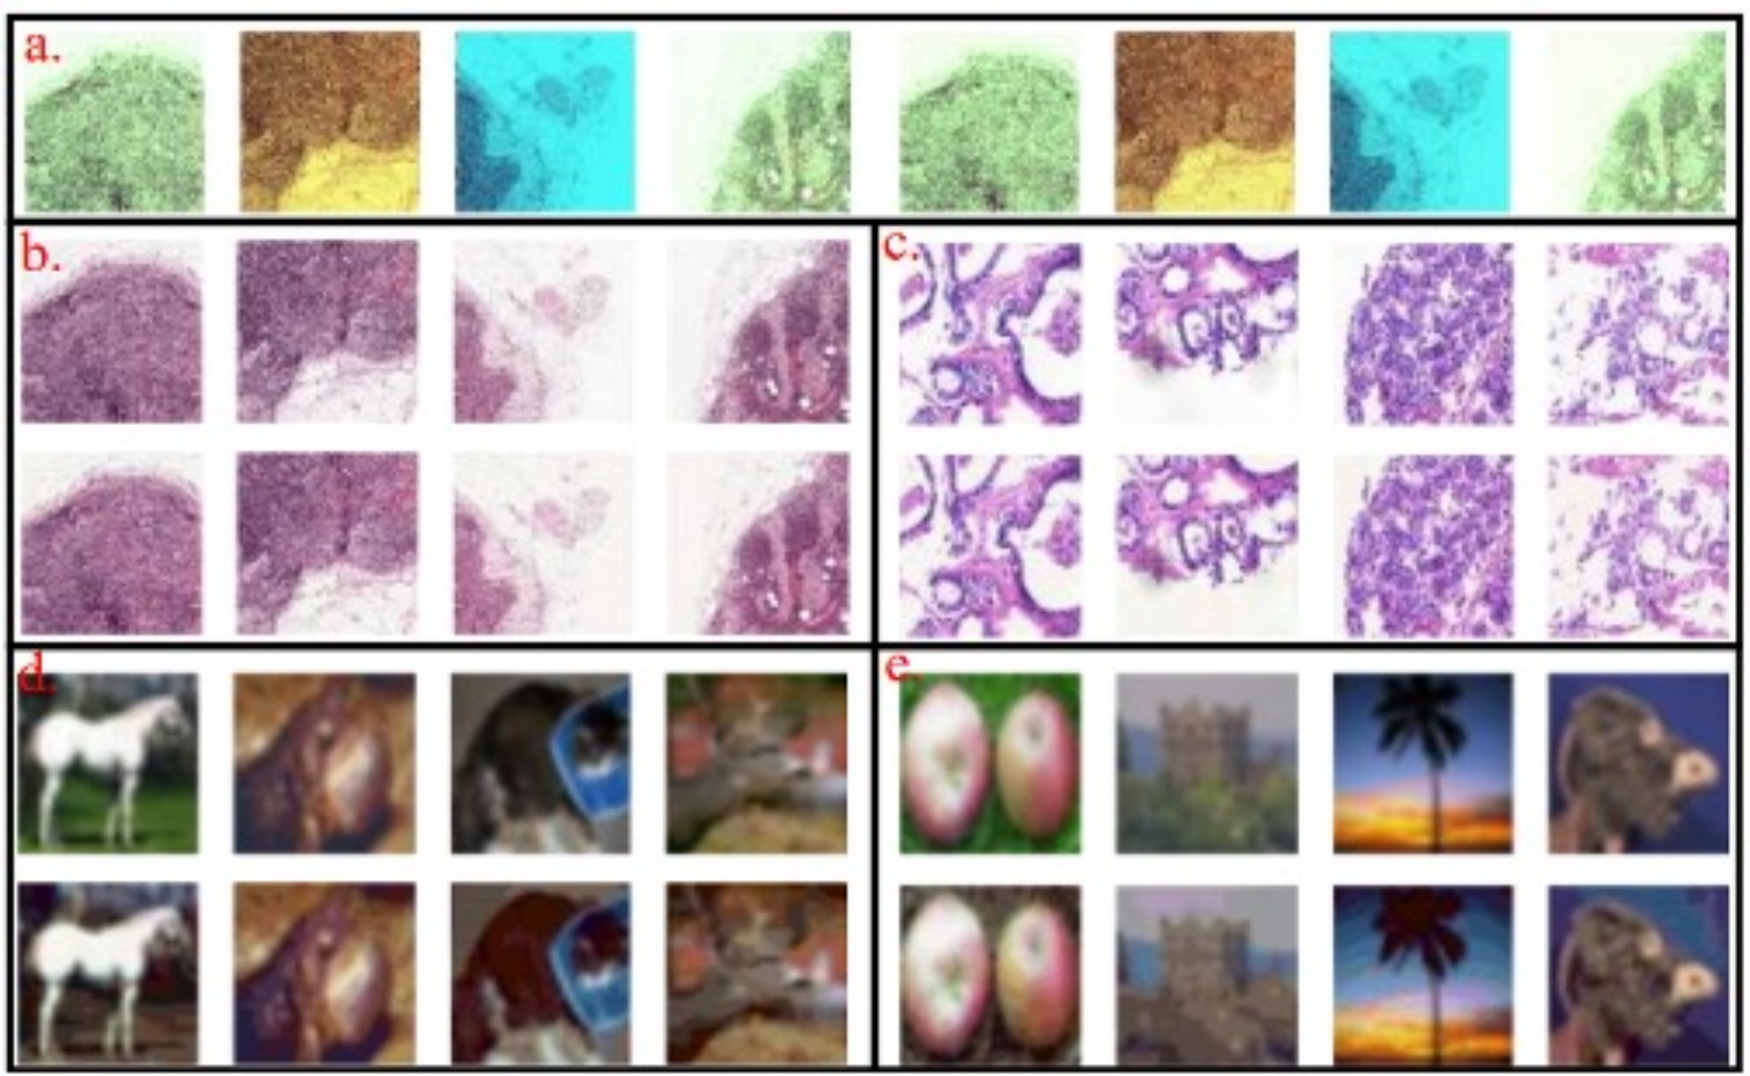
\includegraphics[width=0.5\linewidth]{Figures/new_500_dpi_figures/Example VQVAE images reconstructions and data augmentation.png}
% \caption{Example dataset images with the data augmentation (top row [a]) and the subsequent VQVAE reconstructions for the Camelyon 2016 subset (middle left [b]), UCLA (middle right [c]), cifar 10 (bottom left [d]), cifar 100 (bottom right [e]). The VQVAE was trained on the Camelyon 2016 subset only}
% \end{figure}
% Figure 1. a. shows example Camelyon 2016 subset training images with the colour augmentation applied to the training patches. Figure 1. b. shows the same training image batch without image the data augmentation applied and the reconstruction with the Camelyon 2016 trained VQVAE. Figure 1. c. d. e, show the original and reconstructed testing patches for the UCLA, Cifar 10 and Cifar 100 datasets.

\subsection{Algorithms}
\paragraph{\gls{vqvae} architecture} The \gls{vqvae} architecture uses an encoder, a decoder and a quantizer. The \gls{vqvae} modified this with a secondary encoder and decoder layer. The secondary (top) and primary (bottom) encoder and decoder layers encode for high level and low-level features within the image respectively.

% \begin{figure}
% 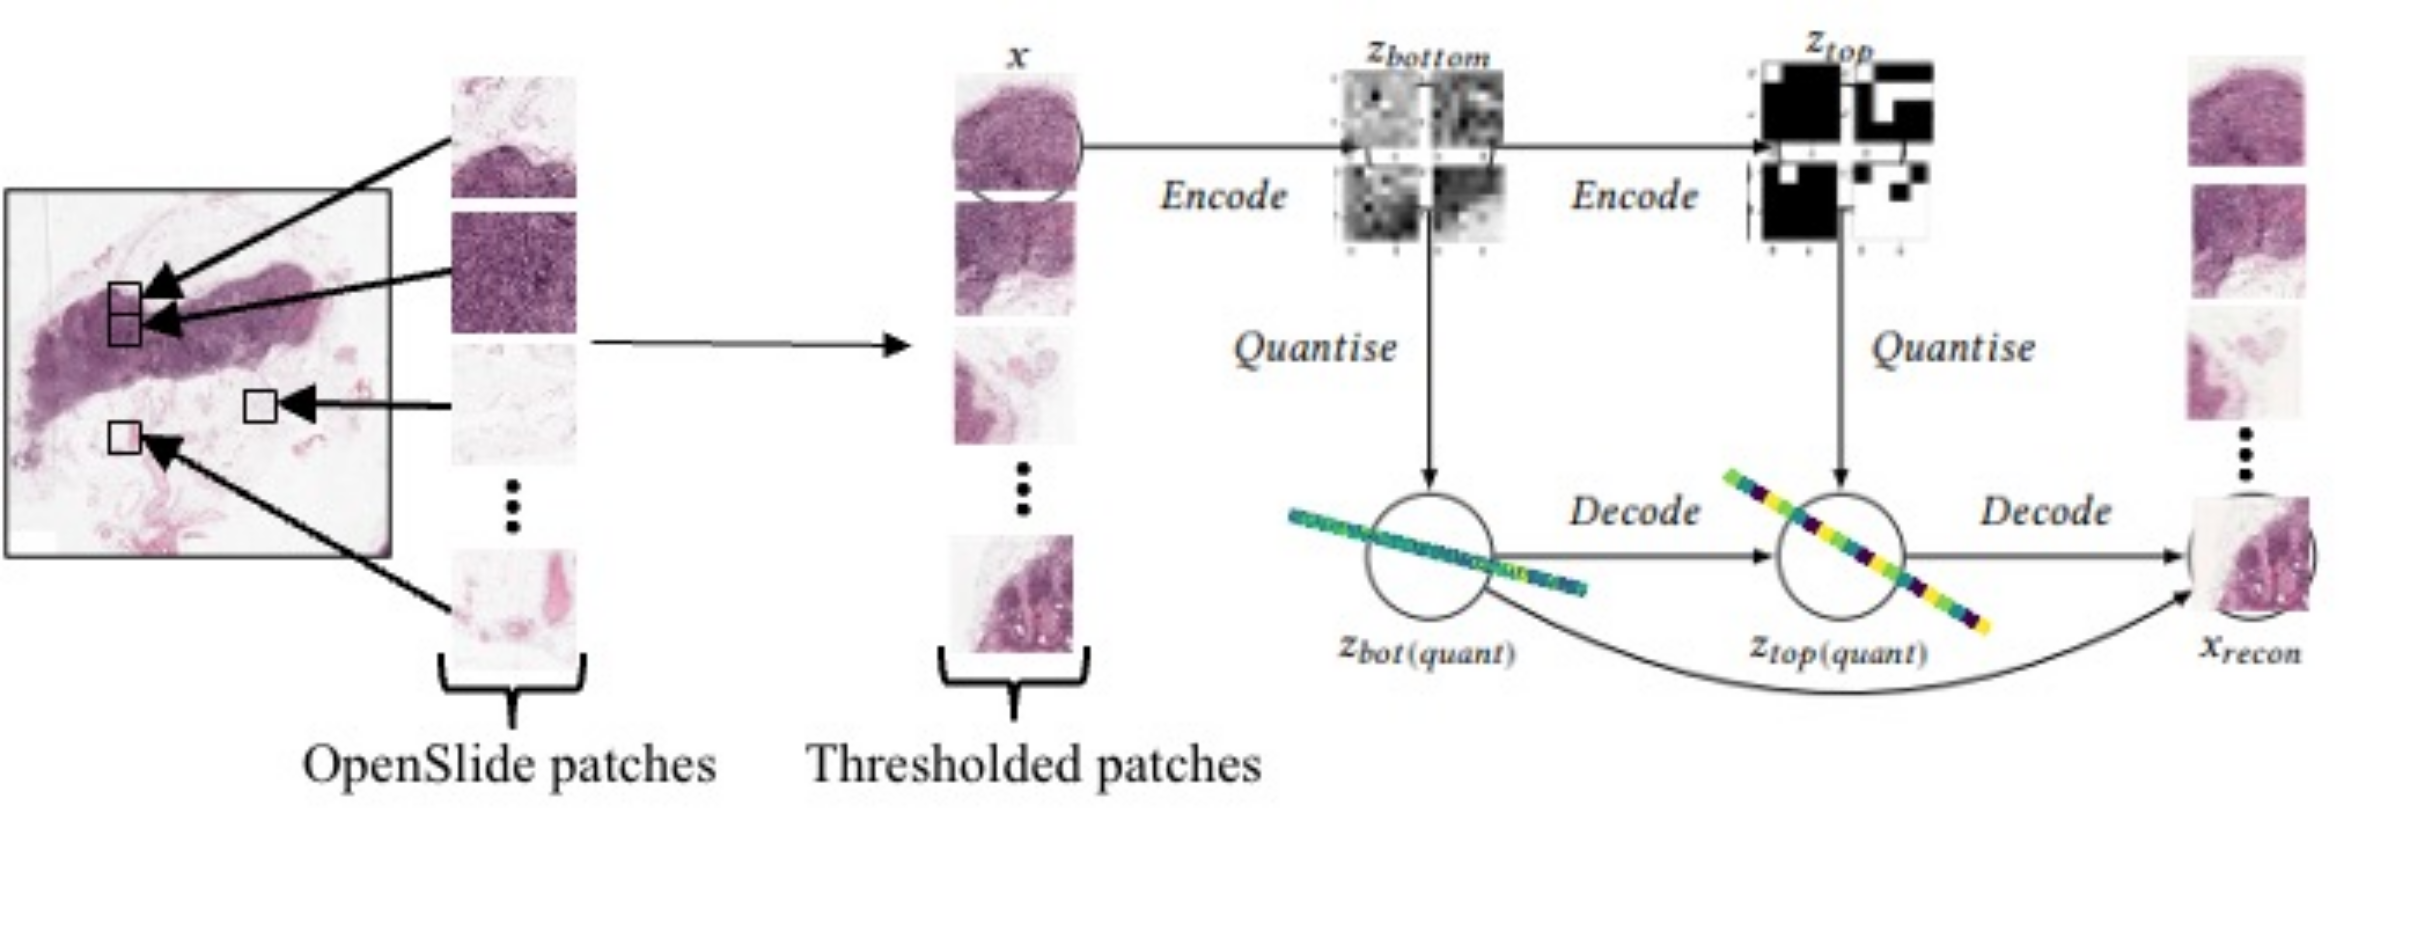
\includegraphics[width=1\linewidth]{Figures/new_500_dpi_figures/Overview diagram VQVAE patch extraction and algorithm.jpeg}
% \caption{Overview of the VQVAE on the Camelyon 2016 subset dataset}
% \end{figure}

\begin{figure}
    \centering
    \resizebox{0.85\linewidth}{!}{
        \tikzfig{latex_figures/VQVAE diagram new/Tikz diagram VQVAE}
    }
    \caption{Overview of the \gls{vqvae} on the Camelyon 2016 subset dataset}
    \label{fig:VQVAE_camelyon_2016_overview_diagram}
\end{figure}

\paragraph{Loss function} The loss function within the \gls{vqvae} has three components, the reconstruction loss, the embedding loss and the commitment loss. The reconstruction loss encodes for the accuracy of the reconstructed image (X') and can be any existing loss function including the mean squared error (MSE). The embedding loss moves the code book embeddings ($Z_{embed(X)}$) towards the normal distribution quantised embeddings ($Z_{embed(quant)}$). The commitment loss moves the embedding ($Z_{embed(quant)}$) towards the image encoded embedding ($Z_{embed(X)}$). \\
    \gls{vqvae} loss=Reconstruction loss+embedding loss-commitment loss
    % VQVAE loss=$MSE(X,X')+(Z_{(embed(X))}-Z_{embed(quant)})-\beta(Z_{embed(quant)}-Z_{(embed(X))} )$
    
\paragraph{\gls{vqvae} training} The \gls{vqvae} implementation was cloned from the GitHub repository (\url{https://github.com/rosinality/vq-vae-2-pytorch}). The default parameters were used for initial training and preliminary testing. The dimension of embeddings and number of embedding parameters were modified to achieve larger or smaller compression of the 512x512x3 image patches. The \gls{vqvae} was trained on the \gls{cam16} subset training data, and then was tested on all other datasets.\\
The default \gls{vqvae} network parameters (in$\_$channel=3, channel=128, n$\_$res$\_$block=2, n$\_$res$\_$channel=32, embed$\_$dim=64, n$\_$embed=512, decay=0.99, loss$\_$function= LossFunction.mean$\_$squared$\_$error) led to a \gls{comprat} of 0.6. The embedding dimension parameter can be changed to change the level of compression within the compressed representation. The embedding dimensions for the embed$\_$dim values of 8, 4, 2 are 4.8:1, 9.6:1 and 19.2:1 respectively for the \gls{comprat} between the compressed representation ($X^{'}$) and the original patch image ($X$). For example within the training within this paper the embedding dimension value of 2 was used to create a 19.2:1 \gls{comprat} with a $R^{((2,128,128))}+R^{((2,64,64))}$ latent space for the $R^{((512,512,3))}$ image data (X).

% \begin{equation}
%     X\in\mathbb{R}^{(512, 512, 3)};\\ X^{quant\_t}\in\mathbb{R}^{(embed\_dim, 128, 128)};\\ X^{quant\_b}\in\mathbb{R}^{(embed\_dim, 64, 64)};\\
%     X'\in\mathbb{R}^{(512, 512, 3)}
%     \label{eq:VQVAEdatashapes}
% \end{equation}

% \begin{equation}
%     VQVAE(X): (encode: X\mapsto (X^{quant\_t}\union X^{quant\_b})) \mapsto (decode: (X^{quant\_t}, X^{quant\_b}\mapsto X'))
%     % & VQVAE(X): decode(encode(X))\mapsto X'
%     \label{eq:VQVAEarchitectureequation}
% \end{equation}

% \begin{align*}
%     % \begin{equation}
%     & encode: X\mapsto (X^{quant\_t}\union X^{quant\_b}) \\
%     & decode: (X^{quant\_t}, X^{quant\_b}\mapsto X') \\
%     & VQVAE(X): decode(encode(X))\mapsto X'
%     \label{eq:VQVAEarchitecture}
%     % \end{equation}
% \end{align*}

    % X∈R^((512,512,3) );X^(quant\_t)∈R^((embed\_dim,128,128) );X^(quant\_b)∈R^((embed\_dim,64,64) );X^'∈R^((512,512,3) ) \\
    % encode: X→〖(X〗^(quant\_t)∪X^(quant\_b)) \\
    % decode: (X^(quant\_t),X^(quant\_b) )→X^' \\
    % VQVAE(X):decode(encode(X))→X^' \\
    
\paragraph{\gls{jpeg}} Two ImageMagick \gls{jpeg} implementations were used: the generic \gls{jpeg} implementation (``magick {source\_file} -strip -quality {quality} {result\_file}''),
 and the \gls{jpeg} 2000 compression (``magick {source\_file} \-strip \-colorspace RGB -define jp2:quality {compression\_ratio} {result\_file}''. \\
 All \gls{jpeg} compression algorithms were run on the same datasets to the \gls{vqvae}, using the same Pytorch dataloaders without data augmentation other than “torchvision.transforms.Resize((512, 512))” for all patches within the pathology datasets. \\
 The \gls{jpeg} compression algorithm compression quality metric was used for every 5\% quality from 2\% to 99\%, this was manually mapped to the compression ratio of the compressed representation. The \gls{jpeg} 2000 used the same numbers from 2 to 99 but within \gls{jpeg} 2000 this value represented the desired compression ratio. The \gls{psnr} and \gls{ssim} values were calculated for all reconstructed images and plotted as a function of the compression ratio for both the \gls{jpeg} and \gls{jpeg} 2000 algorithms.

%%%%% Results – Report of study findings.
\section{Results}
\paragraph{Visual differences between \gls{jpeg} and \gls{vqvae} compression} \gls{jpeg} and \gls{jpeg} 2000 are current compression techniques used within \gls{wsi} storage within hospitals. The compression ratio within these stored images is usually around 15:1 to 20:1 compression ratio. The \gls{vqvae} trained on a 19.2:1 compression ratio reconstructed images were then visually compared to the decompressed images from the \gls{jpeg} compression testing. \\
The reconstructions seemed to be performing better on all datasets compared to the \gls{jpeg} compression at a similar compression level.

\paragraph{Custom data augmentation (colour randomisation)}  The custom colour augmented dataset performed worse in all metrics compared to the \gls{vqvae} trained without the custom data augmentation. The difference in \gls{psnr} (\gls{mean} [\gls{stddev}]) between the \gls{vqvae} trained to the compression ratio of $\sim$19.2 was 1.22 [0.17], -2.2 [0.59], 1.13 [0.42] for the mean and standard deviations of 19.92±1.83, 20.09±1.29, 21.95±1.89 (no colour data augmentation) and 18.70±1.66, 22.29±0.70, 20.82±1.47 (with randomised colour data augmentation) for the \gls{cam16} subset, \gls{ucla} and \gls{intvalset}. The difference in the \gls{ssim} for the \gls{vqvae} trained to the compression ratio of $\sim$19.2 was 0.11 [-0.024], 0.03 [-0.001], 0.07 [-0.009] from the mean and standard deviation of 0.72±0.076, 0.88±0.018, 0.80±0.060 (no colour data augmentation) and 0.61±0.10, 0.85±0.019, 0.73±0.069 (with randomised colour data augmentation) for the \gls{cam16} subset, \gls{ucla} and \gls{intvalset} respectively. \\
The difference within the median and IQR values for the different algorithms is shown in fig. \ref{fig:image_reconstruction_quality_boxplot_for_all_algorithms}.

\paragraph{\gls{jpeg} compression quality quantitative results} The peak signal to noise ratio (\gls{psnr}) and structural similarity (\gls{ssim}) \gls{jpeg} metrics were calculated for the \gls{jpeg} compression. The \gls{psnr} for \gls{jpeg} on the tested pathology datasets dropped significantly from 43 to 32 between the 1:1 and 3:1 compression ratios. The \gls{psnr} for \gls{jpeg} maintained stable with a \gls{psnr} of around 29 after the 5:1 compression ratio.

% \begin{figure}
% \includegraphics[width=1\linewidth]{Figures/new_500_dpi_figures/jpeg ImageMagick compression quality to compression ratio without exif data no title.png}
% % \includegraphics[width=1\linewidth]{Figures/new_500_dpi_figures/jpeg ImageMagick compression quality to compression ratio without exit data.jpeg.jpeg}
% \caption{Imagemagick \gls{jpeg}/\gls{jpeg} 2000 quality flag to compression ratio relationship}
% \end{figure}

\paragraph{\gls{jpeg} vs \gls{vqvae} (mean and standard deviation)} The \gls{psnr} ($\gls{psnr}\in R$) mean and standard deviation for the \gls{ucla} and \gls{cam16} subset with metadata were 28 dB and 28.75 dB. The \gls{psnr} for the \gls{ucla}, \gls{cam16} subset and \gls{intvalset} with \gls{exif} data stripped with imagemagicks -strip flag were 31.50±0.81 dB, 29.70±1.28 dB, 29.91±1.21 dB for the \gls{comprat} of $\sim$19.2:1 for \gls{jpeg} compression. For the \gls{vqvae} compression the \gls{psnr}s \gls{mean} and \gls{stddev} were 20.3±1.09 dB, 19.6 ± 1.77 dB, 21.49 ± 1.83 dB, respectively. \gls{ssim} considers image structure, \gls{psnr} does not. \gls{ssim} ($\gls{ssim}\in [0,1]$) results for the \gls{ucla}, \gls{cam16} subset and \gls{intvalset} were 0.35, 0.35 for \gls{jpeg} with \gls{exif} data. Without \gls{exif} data (imagemagick –strip flag) the \gls{ucla}, \gls{cam16} subset and \gls{intvalset} \gls{ssim} (\gls{mean} ± \gls{stddev}) was 0.84 ± 0.022, 0.83 ± 0.034, 0.80 ± 0.042 for \gls{jpeg} and 0.85 ± 0.022, 0.72 ± 0.072, 0.79 ± 0.056 for the \gls{vqvae} implementation.

% The \gls{psnr} ($\gls{psnr}\in R$) for a Camelyon 2016 subset (10 \gls{wsi} slides) and University of California dataset were 28 dB and 28.75 dB for a compression ratio of $\sim$19.2:1 \gls{jpeg} compression with metadata. For the \gls{vqvae} compression the \gls{psnr}s were 19.6±1.77 dB, 20.3±1.09 dB and 21.49±1.83 dB respectively. \\
% Structural Similarity (\gls{ssim}) considers image structure, \gls{psnr} does not. \gls{ssim} ($\gls{ssim}\in[0,1]$) results for the Camelyon 2016 subset and UCLA datasets were 0.35 and 0.35 for \gls{jpeg} with exif data. The \gls{ssim} (mean±standard deviation) for the Camelyon 2016 subset, UCLA dataset and internal validation training dataset was 0.72±0.076, 0.88±0.018 and 0.80±0.060 ($\sim$19.2:1 compression ratio); 0.75±0.067, 0.87±0.023 and 0.81±0.054 ($\sim$9.6:1 compression ratio); 0.32±0.12, 0.52±0.039, 0.39±0.13 ($\sim$4.8:1 compression ratio) for the \gls{vqvae} implementation trained on the Camelyon 2016 training data subset (9 \glspl{wsi}). With \gls{jpeg} metadata removed from the compression the \gls{psnr} and \gls{ssim} increased to 30.03±1.34, 32.20±0.89, 30.24±1.31 and 0.88±0.025, 0.87±0.018, 0.84±0.038 for the Camelyon 2016 subset, UCLA dataset and an Internal validation set. \gls{jpeg} 2000 compression without metadata outperformed all other compression methods with the \gls{psnr} and \gls{ssim} being 70.55±4.078, 80.04±2.09, 72.86±3.078 and 0.82±0.082, 0.95±0.015, 0.84±0.064 for the Camelyon 2016, UCLA and Internal validation dataset. \\

% \begin{figure}{\linewidth}
%     \centering
%     \includegraphics[width=1\linewidth]{Figures/new_500_dpi_figures/VQVAE data augmentation psnr ssim comparison boxplot.jpeg}
%     \caption{Image reconstruction quality boxplot for \gls{vqvae} with different colour augmentations.}
%   \end{figure}

% \begin {figure}
%   \begin{subfigure}{0.5\linewidth}
%     \centering
%     \includegraphics[width=\linewidth]{Figures/new_500_dpi_figures/VQVAE data augmentation psnr ssim comparison boxplot.jpeg}
%     \caption{Image reconstruction quality boxplot for \gls{vqvae} with different colour augmentations.}
%   \end{subfigure}
%   \begin{subfigure}{0.5\linewidth}
%     \includegraphics[width=\linewidth]{Figures/new_500_dpi_figures/VQVAE data augmentation psnr ssim comparison boxplot With jpeg and jpeg 2000.png}
%     \caption{Image reconstruction quality boxplot for all algorithms}
%     \label{fig:image_reconstruction_quality_boxplot_for_all_algorithms}
%   \end{subfigure}
% \end{figure}

\paragraph{19:1 \gls{jpeg} vs 19.2:1 \gls{vqvae} (medium and interquartile range)} The \gls{psnr} medium and interquartile range for the UCLA and Camelyon 2016 subset and internal validation set are $\sim$21, 20, 21 and $\sim$32, 29, 30 for the \gls{vqvae} and \gls{jpeg} respectively.
The \gls{ssim} medium and interquartile range for the UCLA and Camelyon 2016 subset and internal validation set are $\sim$0.85, 0.72, 0.79 and $\sim$0.84, 0.81, 0.8 for the \gls{vqvae} and \gls{jpeg} respectively.

\begin{figure}
\includegraphics[width=1\linewidth]{Figures/new_500_dpi_figures/VQVAE data augmentation psnr ssim comparison boxplot With jpeg and jpeg 2000.png}
\caption{Image reconstruction quality boxplot for all algorithms}
\label{fig:image_reconstruction_quality_boxplot_for_all_algorithms}
\end{figure}
%%%%% Conclusions - Brief summary and potential implications.

\section{Discussion}
The digitization of the whole slide images requires a large amount of digital storage space. \glspl{autoencoder} and \glspl{vae} have been used in other areas within compression. This shows a possible alternative to the current compression methods used within histopathology. Within histopathology, \gls{jpeg} and \gls{jpeg} 2000 are used by histopathology scanners, including the Aperio scanner range.

% This work focuses on how comparable current variational autoencoders and 

The quantitative metrics for the initial \gls{vqvae} testing showed that the \gls{vqvae} could perform to a degree that was, on average, either comparable or better than \gls{jpeg} within the \gls{ssim} metric, but worse on the \gls{psnr} metric if \gls{jpeg} metadata is saved. If this is removed the \gls{vqvae} \gls{ssim} is lower than that of \gls{jpeg} and \gls{jpeg} 2000. \\
The \gls{psnr} does not consider structural similarity of the two images, the structural similarity (\gls{ssim}) metric does consider the similarity of the structures within the image. 
\glspl{vae} and \glspl{vqvae} have been used successfully for compression and meaning representation tasks within other clinical domains, including within x-ray and CT compression \cite{kwon_appropriate_2020}. \\
As the learnt model was able to generalise between different scanners and different datasets from different locations, the latent space was shown to encode features that represented the image features within the image. Future work aims to understand the representations generated by \glspl{vae} networks, aiming to create clinically useful representations of \gls{wsi} slides and patches while allowing for compression of the pathology images. 

% The poorer results for the \gls{vqvae} implementation on the \gls{psnr} could have been down to a lack of training of the model. The poorer results for the \gls{vqvae} implementation versus the \gls{jpeg} implementations could also have been due to the use of suboptimal training hyper parameters, or possibly the use of a loss function that did not focus on the image reconstruction quality with appropriate metrics (\gls{psnr} or \gls{ssim} rather than MSE).
% % , with the latent space embedding representations being favoured or balanced over the reconstruction accuracy metrics of \gls{psnr} or \gls{ssim}.
% % A full hyperparameter search for the \gls{vqvae} network was not performed to gain the optimal parameters for the network compression.
% % More \gls{wsi} slides could have been used for training and testing of the data, using multiple datasets should mitigate the generalisability of this issue. As the metrics were done on a per patch basis, this may not be fully transferable to a whole slide image compression metric, further research would have to be done to confirm this.


% The \gls{jpeg} and \gls{jpeg} 2000 implementations optimise towards an \gls{ssim} or \gls{psnr} value, whereas the loss function for the trained \gls{vqvae} was focussed on embedding similarity towards the normal distribution sample with reconstruction loss being in the form of the MSE. 

% were focussed on a euclidian difference between the embeddings and the normal distribution sample, as well as the MSE loss. Therefore it may be possible to optimse the \gls{vqvae} towards attaining a good \gls{ssim} value by encorporating this within the loss function itself.

\paragraph{Limitations} The tested \glspl{vae} networks may have been mapping too much towards the reconstructed image, rather than ensuring mapping to the normal distribution feature representations, therefore ignoring the normal distribution feature mapping in favour of minimizing the reconstruction image accuracy, latent space testing and visualisation is aimed to be done in the future. \\
The poorer results for the \gls{vqvae} implementation on the \gls{psnr} could have been down to a lack of training of the model (epochs=500), however training new models on 2000 epochs did not change the results significantly. The poorer results for the \gls{vqvae} implementation versus the \gls{jpeg} implementations could also have been due to the use of suboptimal training hyper parameters, or possibly the use of a loss function that did not focus on the image reconstruction quality, with the latent space embedding representations being favoured or balanced over the reconstruction accuracy metrics of \gls{psnr} or \gls{ssim}. \\
A full hyperparameter search for the \gls{vqvae} network was not performed to gain the optimal parameters for the network compression. \\
More \gls{wsi} slides could have been used for training and testing of the data, using multiple datasets should mitigate the generalisability of this issue. As the metrics were done on a per patch basis, this may not be fully transferable to a whole slide image compression metric, further research would have to be done to confirm this.

\paragraph{Future work} Future research could focus on merging of the data with \glspl{vae} and other techniques, for example, normalizing flows and manifolds. \\
If the compression of \glspl{vae} could compete with existing methods, the compression would allow for the compressed representation to contain meaning within the latent features, possibly allowing for abstraction of clinically relevant features for faster analysis of the biopsy tissue contained on the slide. \\
Future research aims to compare the compression error type to subjective image quality and performance metrics, as well looking at the application of the network on uncompressed data. \\

% Competing interests
\section{Compliance with Ethical Standards}
This work was carried out under regional ethical approval (Leeds West REC,  reference 05/Q1205/220).

% Authors' contributions
\section{Compliance with EPSRC open access requirements}
In compliance with the UKRI and EPSRC open access requirements, all publishable material and code has been made available. The internal validation dataset contains patient data and so cannot be made publicly available. The code and data used for the experimentation can be found at \url{www.github.com/Jjk422/Journal-of-Pathology-Informatics-compression-paper-2022}.

% Acknowledgements
\section{Acknowledgements}
JK is funded via the Leeds University Centre for Doctoral Training (CDT) for AI in medical diagnosis and care with a grant from EPSRC (Project no. 2271095). \\
DT and AW are funded by National Pathology Imaging Co-operative, NPIC (Project no. 104687), supported by a £50m investment from the Data to Early Diagnosis and Precision Medicine strand of the government’s Industrial Strategy Challenge Fund, managed and delivered by UK Research and Innovation (UKRI).

% References
\section{References}



% \section{The Elsevier article class}

% \paragraph{Installation} If the document class \emph{elsarticle} is not available on your computer, you can download and install the system package \emph{texlive-publishers} (Linux) or install the \LaTeX\ package \emph{elsarticle} using the package manager of your \TeX\ installation, which is typically \TeX\ Live or Mik\TeX.

% \paragraph{Usage} Once the package is properly installed, you can use the document class \emph{elsarticle} to create a manuscript. Please make sure that your manuscript follows the guidelines in the Guide for Authors of the relevant journal. It is not necessary to typeset your manuscript in exactly the same way as an article, unless you are submitting to a camera-ready copy (CRC) journal.

% \paragraph{Functionality} The Elsevier article class is based on the standard article class and supports almost all of the functionality of that class. In addition, it features commands and options to format the
% \begin{itemize}
% \item document style
% \item baselineskip
% \item front matter
% \item keywords and MSC codes
% \item theorems, definitions and proofs
% \item lables of enumerations
% \item citation style and labeling.
% \end{itemize}

% \section{Front matter}

% The author names and affiliations could be formatted in two ways:
% \begin{enumerate}[(1)]
% \item Group the authors per affiliation.
% \item Use footnotes to indicate the affiliations.
% \end{enumerate}
% See the front matter of this document for examples. You are recommended to conform your choice to the journal you are submitting to.

% \section{Bibliography styles}

% There are various bibliography styles available. You can select the style of your choice in the preamble of this document. These styles are Elsevier styles based on standard styles like Harvard and Vancouver. Please use Bib\TeX\ to generate your bibliography and include DOIs whenever available.

% Here are two sample references: \cite{Feynman1963118,Dirac1953888}.

% \nocite{*}

\bibliography{references.bib}

% Figure legends (if any)
% \section{Figure legend}


% Tables and captions (if any)
\section{Tables and captions}
\begin{table}[!h]
    \centering
    \begin{tabular}{p{0.15\linewidth} p{0.1\linewidth} p{0.1\linewidth} p{0.25\linewidth} p{0.24\linewidth}}
    \toprule
    \textbf{Algorithm} & \textbf{Has meta data} & \textbf{Test dataset} & \textbf{\gls{psnr}} & \textbf{\gls{ssim}} \\
    \bottomrule
    % & jpeg; meta\\
    % \midrule
    jpeg & Yes & \gls{cam16} & 28 & 0.35 \\
    & & \gls{ucla} & 28.75 & 0.35 \\
    \bottomrule
    
    % & jpeg; no-meta & \\
    % \midrule
    jpeg & No & \gls{cam16} & 30.03±1.34 (29.8867, 30.1733) & 0.88±0.025 (0.8773, 0.8827) \\
    & & \gls{ucla} & 32.20±0.89 (31.9687, 32.4313) & 0.87±0.018 (0.8653, 0.8747) \\
    & & \gls{intvalset} & 30.24±1.31 (30.1816, 30.2984) & 0.84±0.038 (0.8383, 0.8417) \\
    \bottomrule
    
    % & j2000; no-meta & \\
    % \begin{tabular}{l l l}
    % \midrule
    jpeg 2000 & No & \gls{cam16} & 70.55±4.078 (70.1140, 70.9860) & 0.82±0.082 (0.8112, 0.8288) \\
    & & \gls{ucla} & 80.04±2.09 (79.4969, 80.5831) & 0.95±0.015 (0.9461, 0.9539) \\
    & & \gls{intvalset} & 72.86±3.078 (72.7229, 72.9971) & 0.84±0.064 (0.8371, 0.8429) \\
    \bottomrule
    % \caption{jpeg/jpeg 2000 (CR: $\sim$19) metrics}
    \end{tabular}
    \caption{jpeg/jpeg 2000 (Compression ratio: $\sim$19.2) metrics. Mean±Standard deviation (t-test: 95\% confidence interval)}
    \label{tab:my_label}
\end{table}

% Description of additional data files (if any)
\section{Additional data files}
\paragraph{Code availability} Code can be found at \url{https://github.com/Jjk422/Digipath-WSI-compress-VQVAE}.
\paragraph{Data availability} Data for the Camelyon 2016 dataset can be found at \url{https://camelyon16.grand-challenge.org/}, \gls{ucla} data can be found at \url{https://bioimage.ucsb.edu/research/bio-segmentation}. The internal validation set contains patient data and so cannot be publicly shared.

\end{document}